% -*- root: ../main.tex -*-
%!TEX root = ../main.tex
% this file is called up by main.tex
% content in this file will be fed into the main document
% vim:textwidth=80 fo=cqt

At this  stage, it must  be recalled that the  purpose of developing  the system
identification electrolyte  model was  to mitigate the  poor performance  of the
basic  \gls{spm} at  C-rates above  0.5C (see~\cref{subsec:simresultsbasicspm}).
This sub-optimal performance was attributed  to the lack of electrolyte dynamics
in  the  basic  \gls{spm}.  The   performance  of  the  newly  developed  system
identification model has been proved to be  superior to the current state of the
art. The next step  is to embed this electrolyte model  into the basic \gls{spm}
so as to  obtain a composite \gls{spm}. The performance  of this composite model
is evaluated to ascertain its suitability towards online implementation.

\subsection{Computation of electrolyte overpotential}

In~\cref{subsec:simresultsbasicspm}, it  was shown that in  the basic \gls{spm},
the computation of the cell's \gls{soc}  is of sufficient accuracy. However, its
terminal voltage is  far from the true  value as computed by  a \gls{p2d} model.
This mismatch between \gls{soc} and  terminal voltage hinders the suitability of
the basic \gls{spm} as the plant model in online state estimation applications.

The missing component in the terminal voltage computation of the basic \gls{spm}
is  the  contribution from  the  electrolyte  overpotential  term. This  is  the
potential difference in  the entire electrolyte \ie{}  the electrolyte potential
at the positive current collector interface with respect to that at the negative
current collector interface.


As discussed in~\cref{sec:electrolyteinclusion}, using  the equation proposed by
Prada~\etal~\cite{Prada2012}, the  overpotential in the electrolyte  is computed
as
\begin{align}
    \quad \phi_\epos - \phi_\eneg &= (1-t_{+}^0) \frac{2RT}{F}\ln \frac{c_\text{e,\tiny pos/cc}}{c_\text{e,\tiny neg/cc}}\nonumber\\
    {} &\quad -\frac{I}{2 A}\left(\frac{l_\text{neg}}{\kappa_\text{eff,neg}} + 2 \frac{l_\text{sep}}{\kappa_\text{eff,sep}} + \frac{l_\text{pos}}{\kappa_\text{eff,pos}}\right) \tag{\cref{eq:electrolytepdwithce} revisited}
\end{align}

\Cref{eq:electrolytepdwithce} consists of two distinct terms ---
\begin{enumerate*}[label=\roman*)]
    \item a diffusion overpotential due to concentration gradient in the electrolyte, and
    \item an ohmic resistance term that is dependent upon
        \begin{enumerate*}[label=\itshape\alph*\upshape)]
            \item the instantaneous value of applied current,
            \item the thicknesses of the three cell regions, and
            \item the effective ionic conductivity in each of the three regions. %which in-turn depends on ionic concentration,.
        \end{enumerate*}
\end{enumerate*}

The ohmic  loss term  of~\cref{eq:electrolytepdwithce} needs  to be  examined in
closer detail.  The dependence of  this term  on instantaneous load  current and
cell thicknesses  can be accounted  in a straightforward manner.  However, there
are ambiguities  in computing the  effective ionic  conductivity in each  of the
three cell regions. The effective value of ionic conductivity in the electrolyte
depends on its intrinsic conductivity, the Bruggeman constants and porosities of
each  of  the three  regions.  The  intrinsic electrolyte  conductivity  in-turn
depends on the electrolyte concentration.

Ambiguities   arise   in  interpreting   the   value   of  ionic   concentration
to   be    used   for   computation   of    electrolyte   concentration.   Since
\cref{eq:electrolytepdwithce}  deals  with  overall potential  drop  across  the
entire  length of  the cell,  the concentration  used for  computing electrolyte
conductivity could,  for example be  that at the respective  current collectors.
This concept however  introduces inconsistencies with the  separator term. Using
the  separator concentration  from one  of the  electrode interfaces  introduces
unequal  weighting  in this  computation.  If  the  ionic concentration  at  the
midpoint of the separator is used, this scheme becomes inconsistent with that at
the  two current  collectors. Another  possibility for  computing the  effective
conductivity in a  cell region is to  use the mean of the  concentration in that
region. However, since the mean is nothing but a simple statistical first moment
is  equally influenced  by the  entire  concentration profile  within each  cell
region. This is questionable given that the electrolyte overpotential across the
entire cell thickness  is most likely governed by the  conductivities at the two
current  collector interfaces.  Some form  of weighted  mean could  be conjured,
wherein the  current collector locations  are given  the highest weight  and the
separator locations the  least weight. However, finding the  weights becomes yet
another  exercise and  from the  engineering perspective  of computing  these in
real-time, seems to be in the realm of diminishing returns.

In  published  literature,  only  a  cursory  treatment  has  been  accorded  to
the  aforementioned  ambiguities.  In  Prada~\etal~\cite{Prada2012},  the  usage
of  initial concentrations  is  used  to only  introduce  the  concept of  ohmic
resistance  in that  article.  However,  the author  of  this  thesis wishes  to
extend  this  concept further.  In  the  simulations  conducted by  this  thesis
author, it  became clear  that the  dependence on  applied current  was required
in  order to  obtain  reasonable accuracies.  Computing  mean of  concentrations
in  cell  regions for  calculation  of  ionic  conductivities  led to  a  biased
computation of overpotentials.  Therefore, this author decided to  use the value
of  initial concentration  for the  computation of  ionic conductivities  in the
current-dependent  contribution  to  electrolyte  overpotential  throughout  the
entire time horizon considered.

Hence, as per the adopted scheme~\cref{eq:electrolytepdwithce} gets modified as
\begin{align}
    \quad \phi_\epos(t) - \phi_\eneg(t) & = (1-t_{+}^0) \frac{2RT}{F}\ln \frac{c_\text{e,\tiny pos/cc}(t)}{c_\text{e,\tiny neg/cc}(t)}\nonumber \\
    {}                             &\quad -\frac{I}{2 A}\left(\frac{l_\text{neg}}{\kappa_\text{eff,neg}\left(c_\text{e}\left(0\right)\right)} + 2
    \frac{l_\text{sep}}{\kappa_\text{eff,sep}\left(c_\text{e}\left(0\right)\right)} +
\frac{l_\text{pos}}{\kappa_\text{eff,pos}\left(c_\text{e}\left(0\right)\right)}\right)\label{eq:electrolytepdwithcenew}
\end{align}
wherein  the time-dependent terms are explicitly shown in the notation.

Using~\cref{eq:electrolytepdwithcenew} for electrolyte overpotential computation
has an  important implication. The  two-pronged influence of  the time-dependent
electrolyte concentration on the electrolyte overpotential, \viz
\begin{enumerate*}[label=\itshape\alph*\upshape)]
    \item a direct influence in the form of concentration dependent diffusion polarisation, and
    \item an indirect influence through its use in ionic conductivity calculations
\end{enumerate*}
has  now  been  reduced  to  just   one.  This  implies  the  results  from  the
system  identification   model  are  now   required  only  in  the   first  term
of~\cref{eq:electrolytepdwithcenew}.

In the light of the decision of use the (constant) initial concentration for the
ohmic term, it is natural to question the gains from the circuitous route of the
system  identification  exercise that  was  undertaken  to obtain  the  improved
electrolyte model. Therefore,  it is imperative to quantify  the relative weight
of  the  concentration  dependent  diffusion resistance  compared  to  the  bulk
solution resistance.

\begin{figure}[!htbp]
    \centering
    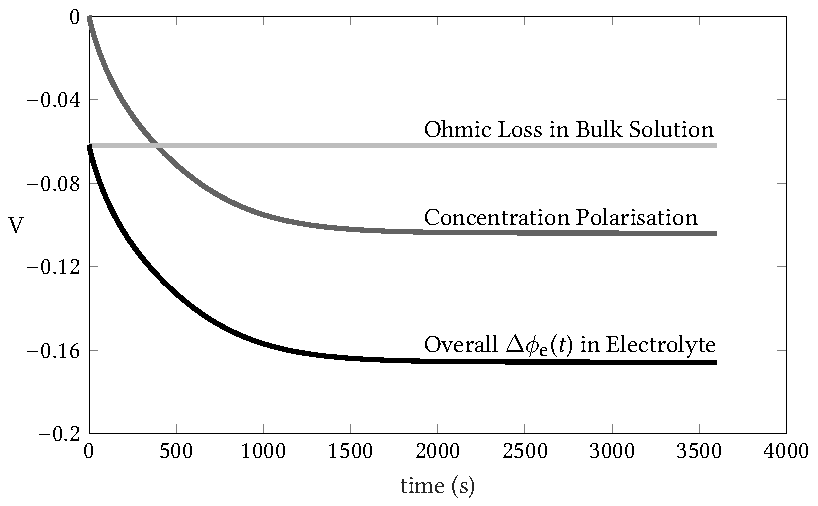
\includegraphics{contribution_to_phie_1C.pdf}
    \caption[%
    Contribution to electrolyte overpotential from the gradient-induced polarisation
    term and the bulk solution resistance term for a 1C discharge
    ]%
    {%
        Contribution to the overpotential in the electrolyte from each of the
        two terms in~\cref{eq:electrolytepdwithcenew} for a 1C discharge. The
        bulk solution resistance is approximated as a constant value determined
        by the equilibrium initial concentration. The concentration dependent
        polarisation term governs the dynamic behaviour of the overall
        overpotential. Furthermore, this gradient-induced diffusion resistance
        has a strong contribution to the steady state, higher than the bulk
        solution resistance and cannot be neglected without introducing
        significant errors.
}%
\label{fig:contributiontophiefromtwoterms}
\end{figure}

\Cref{fig:contributiontophiefromtwoterms} shows the  contribution to the overall
potential drop  $\phi_\text{e,pos}$ and  $\phi_\text{e,neg}$ in  the electrolyte
from  each  of  the  two  terms  in~\cref{eq:electrolytepdwithcenew}  for  a  1C
discharge. The bulk  solution resistance is constant owing to  the fact that the
initial  electrolyte concentration  is  used in  computing  the effective  ionic
conductivities in the three regions of  the cell. The gradient induced diffusion
polarisation term, however has a stronger contribution in both the transient and
steady  state. The  entire dynamics  of the  overall potential  drop during  the
transient  phase is  governed by  this concentration-dependent  term, while  its
steady state contribution  is in-fact higher than the  bulk solution resistance.
The  constant  ohmic resistance  term  merely  provides  a non-zero  offset  for
the  electrolyte  solution  overpotential.  In questioning  whether  the  system
identification exercise was indeed worthwhile,  if the concentrations in the two
current collectors had not been computed  at each time-step, then this diffusion
polarisation  term  would  become  zero.  This is  because,  the  numerator  and
denominator in~\cref{eq:electrolytepdwithcenew} would have to be retained at the
initial concentration, leading to a unit  ratio whose natural logarithm is zero.
Therefore, it  is clear  that computing  the concentrations  at the  two current
collectors  through system  identification has  indeed helped  in improving  the
modelling accuracy.

Having established the relative  importance of computing the diffusion-dependent
polarisation   overpotential,   the   next    question   to   be   answered   is
whether  the  constant  approximation  for   the  bulk  solution  resistance  is
indeed   appropriate.   It  also   remains   to   be   seen  if   the   accurate
computation   of  the   ionic   concentration   through  system   identification
(see~\cref{sec:perfanalysisnewmodel}) has  translated into a  similarly accurate
computation of  electrolyte overpotential. This  is answered by a  comparing the
electrolyte overpotential computed by the  system identification model with that
obtained from the \gls{p2d} model.

\begin{figure}[!htbp]
    \centering
    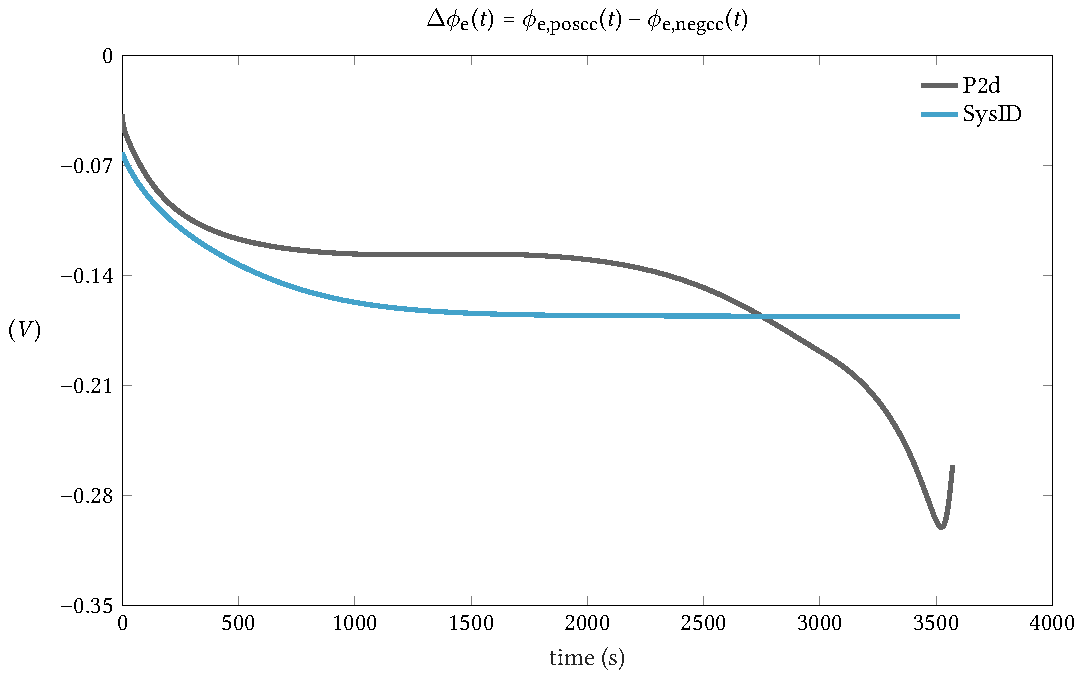
\includegraphics{phie_delta_cnst_1C.pdf}
    \caption{%
        Comparison   of   electrolyte overpotential   computed
        by   the   \gls{p2d}  model   and   the   system  identification   model
        (using~\cref{eq:electrolytepdwithcenew}) for a 1C discharge. During the
        transient phase, the profile obtained by the system identification model
        closely matches that of the \gls{p2d}  model. The mismatch in the
        initial overpotential  does not  arise to  the use  of a  constant
        concentration for the bulk resistance contribution, since
        at equilibrium this value is exact and not an approximation. Past the
        initial transient, accuracy of the system identification model
        degrades. This can be explained by its analogous behaviour for
        concentration computation in the \glsfmtlong{qss} (see~\cref{subsec:tfquadceconstcurrinput}).
    }%
    \label{fig:phiedeltacnst1C}
\end{figure}

\begin{figure}[!htbp]
    \centering
    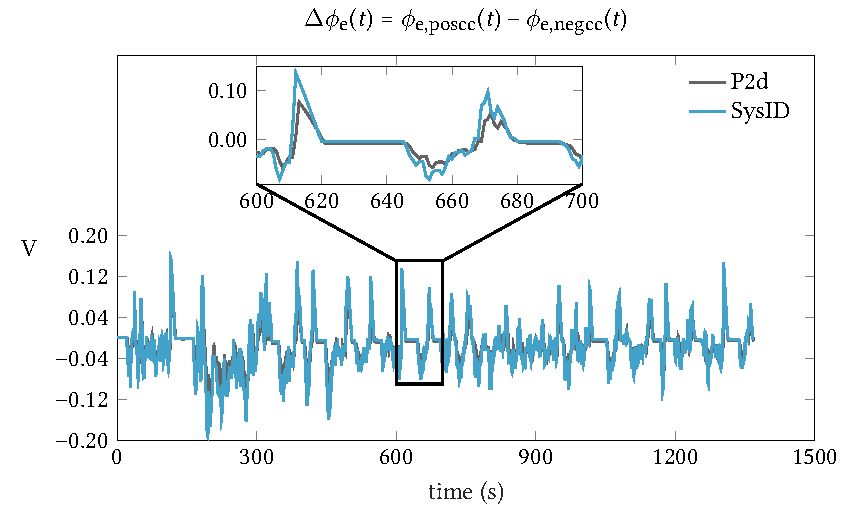
\includegraphics{phie_delta_udds.pdf}
    \caption{}
    \label{}
\end{figure}


% Referring   to~\cref{eq:posoverpotential}  and~\cref{eq:negoverpotential},   the
% reaction overpotential in each of the two porous electrode regions is given by
% \begin{align}
%     η_\text{pos} &= ϕ_\spos - ϕ_\epos - U_\text{pos} \label{eq:posoverpotentialoverall} \\% \tag{\cref{eq:posoverpotential} revisited}\\
%     η_\text{neg} &= ϕ_\sneg - ϕ_\eneg - U_\text{neg} \label{eq:negoverpotentialoverall} %\tag{\cref{eq:negoverpotential} revisited}
% \end{align}
% wherein the contribution from the electrolyte potential terms $ϕ_\epos$ and $ϕ_\eneg$ are not neglected.

% Subtracting~\cref{eq:negoverpotentialoverall}
% from~\cref{eq:posoverpotentialoverall}
% \begin{align}
%  η_\text{pos} - η_\text{neg} &= \underbrace{ϕ_\spos - ϕ_\sneg}_{V_\text{cell}} - ϕ_\epos + ϕ_\eneg - U_\text{pos} + U_\text{neg}\\
% \shortintertext{whose rearrangement yields}
% V_\text{cell} &= η_\text{pos} - η_\text{neg} + \underbrace{ϕ_\epos - ϕ_\eneg}_{\Delta \phi_\text{e}} + U_\text{pos} - U_\text{neg}
% \end{align}

